\documentclass{beamer}
\usepackage[utf8]{inputenc}
\usepackage[UKenglish]{babel}
\usepackage[UKenglish]{isodate}
\usepackage[style=verbose]{biblatex}
\usepackage{amsmath}
\usepackage{tikz}

\usetikzlibrary{shapes}
\usetikzlibrary{arrows}
\usetikzlibrary{arrows.meta}

\beamertemplatenavigationsymbolsempty
\addbibresource{talk.bib}
\DeclareRobustCommand{\stirling}{\genfrac\{\}{0pt}{}}

\author{Paulius Dilkas}
\title{Symmetric Weighted First-Order Model Counting and Factorial-Like Functions}
\date{}

\begin{document}
\addtobeamertemplate{block begin}{\setlength\abovedisplayskip{0pt}}

\maketitle

\begin{frame}{WFOMC: State of the Art}
  I'm excluding techniques that are restricted to two variables and purely
  theoretical results.
  \begin{enumerate}
  \item \cite{DBLP:conf/nips/KazemiKBP16}
    \begin{itemize}
    \item generic domain recursion (implementation unavailable)
    \end{itemize}
  \item \alert{Forclift}: \cite{DBLP:conf/ijcai/BroeckTMDR11}
    \begin{itemize}
    \item somewhat restrictive but well-developed
    \end{itemize}
  \item \alert{L2C}: \cite{DBLP:conf/kr/KazemiP16}
    \begin{itemize}
    \item very basic
    \end{itemize}
  \item \alert{Alchemy}: \cite{DBLP:conf/aaai/DomingosKPRS06}
    \begin{itemize}
    \item old, mostly focused on approximations
    \end{itemize}
  \end{enumerate}
\end{frame}

\begin{frame}{Counting (Unweighted) Functions: Currently Unliftable (1)}
  \cite{stanley2011enumerative}
  \begin{block}{Functions $M \to N$ (let $|M| = m$ and $|N| = n$)}
    Theory:
    \begin{align*}
      \forall x \in M. \forall y, z \in N. &P(x, y) \land P(x, z) \Rightarrow y=z \\
      \forall x \in M. \exists y \in N. &P(x, y)
    \end{align*}
    Answer: $n^m$.
  \end{block}
  \begin{block}{Injections}
    Theory:
    \begin{align*}
      \forall x \in M. \forall y, z \in N. &P(x, y) \land P(x, z) \Rightarrow y=z \\
      \forall x \in M. \exists y \in N. &P(x, y) \\
      \alert{\forall w, x \in M. \forall y \in N.} &\alert{P(w, y) \land P(x, y) \Rightarrow w=x}
    \end{align*}
    Answer: $n^{\underline{m}} = n \cdot (n-1)\cdots(n-m+1)$ if $m \le n$ and $0$ otherwise (for positive $m$ and $n$).
  \end{block}
\end{frame}

\begin{frame}{Counting (Unweighted) Functions: Currently Unliftable (2)}
  \begin{block}{Surjections}
    Theory:
    \begin{align*}
      \forall x \in M. \forall y, z \in N. &P(x, y) \land P(x, z) \Rightarrow y=z \\
      \forall x \in M. \exists y \in N. &P(x, y) \\
      \alert{\forall y \in N. \exists x \in M.} &\alert{P(x, y)}
    \end{align*}
    Answer: $n!\stirling{m}{n} = \sum_{i=0}^n (-1)^i\binom{n}{i}(n-i)^m$.
  \end{block}
  \begin{block}{Bijections}
    Theory:
    \begin{align*}
      \forall x \in M. \forall y, z \in N. &P(x, y) \land P(x, z) \Rightarrow y=z \\
      \forall x \in M. \exists y \in N. &P(x, y) \\
      \alert{\forall w, x \in M. \forall y \in N.} &\alert{P(w, y) \land P(x, y) \Rightarrow w=x} \\
      \alert{\forall y \in N. \exists x \in M.} &\alert{P(x, y)}
    \end{align*}
    Answer: $n!$ if $m=n$.
  \end{block}
\end{frame}

\begin{frame}{Counting (Unweighted) Functions: Currently Unliftable (3)}
  \begin{block}{Partial functions}
    Theory: $\forall x \in M. \forall y, z \in N. P(x, y) \land P(x, z)
    \Rightarrow y=z$

    Answer: $(n+1)^m$.
  \end{block}
  \begin{block}{Partial injections}
    Theory:
    \begin{align*}
      \forall x \in M. \forall y, z \in N. &P(x, y) \land P(x, z) \Rightarrow y=z \\
      \forall w, x \in M. \forall y \in N. &P(w, y) \land P(x, y) \Rightarrow w=x
    \end{align*}
    My answer: $\sum_{k=0}^{\min\{m, n\}} k!\binom{m}{k}\binom{n}{k}$.

    \pause
    \alert{Answer found by Forclift:}
    \[
    f(m, n) =
    \begin{cases}
      1 & \text{if } m = 0 \\
      \sum_{k=0}^n \binom{n}{k} [k < 2] f(m-1, k) & \text{otherwise.}
    \end{cases}
    \]
    (exponential...)
  \end{block}
\end{frame}

\begin{frame}{Conceptual Plan of Action}
  \centering
  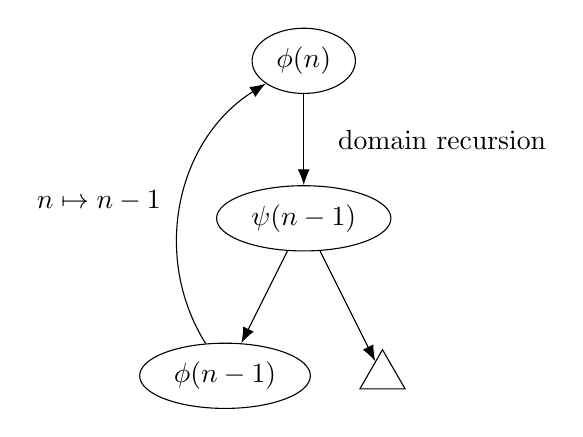
\begin{tikzpicture}[triangle/.style = {regular polygon, regular polygon sides=3}]
    \node[draw,ellipse] (a) at (0, 0) {$\phi(n)$};
    \node[draw,ellipse] (b) at (0, -2) {$\psi(n-1)$};
    \node[draw,ellipse] (c) at (-1, -4) {$\phi(n-1)$};
    \node[draw,triangle] (d) at (1, -4) {};
    \draw[-{Latex[length=2mm]}] (a) -- (b) node [midway,xshift=50] {domain recursion};
    \draw[-{Latex[length=2mm]}] (b) -- (c);
    \draw[-{Latex[length=2mm]}] (b) -- (d);
    \draw[-{Latex[length=2mm]}] (c) to [bend left=45] node [midway,xshift=-30] () {$n \mapsto n-1$} (a);
  \end{tikzpicture}
\end{frame}

\begin{frame}{Remarks on the Implementation}
  \begin{itemize}
  \item WMC computation now loops over the graph.
  \item We propagate information (e.g., for smoothing) in reverse until convergence.
  \item Need a good way to recognise equivalent/isomorphic theories.
  \item Need to be careful about the order of operations:
    \begin{itemize}
    \item Create a (half-empty) vertex $v$.
    \item Add it to the cache.
    \item Recurse on its direct successors $S$.
    \item Add the edges from $v$ to $S$.
    \item After the graph is constructed, propagate information through the
      graph that would otherwise cause infinite loops.
    \end{itemize}
  \end{itemize}
\end{frame}

\end{document}
